% chap4.tex - Week 4
\cleardoublepage
%\phantomsection
\chapter{Week 4}
\section{Day 1 - ``Finally we're getting somewhere''}
\subsection{Planting trees}

Tamagoyaki Inc have now realised that they have to take these things slow and steady if they want to implement a stable and robust system.  This week, they are going to start actually using branches and merging in changes, probably one of the largest topics to cover when doing any type of collaborative development.  

\begin{trenches}
``Dude!'' shouted Eugene from across the office.  ``Dude!!'' he repeated.

No one looked up and the hum of the computers seemed to drown out the mumours of voices and clicking of keys.  

``Dud\ldots'' He was cut off by another voice.  It was Klaus.

``Maybe if you gave us some indication of who you were addressing Eugene,'' said Klaus in his usual matter-of-factly tone, ``we may actually be able to help you.''  

``John!''  Shouted Eugene, as if ignoring Klaus entirely.  The manager hadn't looked up from his monitor as he had advised the tools guy and he now sat there continuing to type with one hand, the other reaching over and yanking out the earbud that was playing a droning beat in John's ear.

``Ouch!'' said John startled.

``Dork wants you,'' said Klaus, using his pet name for Eugene.  

John walked over to Eugene.  ``Sup?!''

``I don't get branches,'' said the developer.  ``I mean I don't get what the heck they do, why I would ever want to use them, and how are they even different to tags anyway?''
\end{trenches}

First we should probably start off by describing what branches are and what they can be used for.  In Git, a branch is just a pointer to a commit in the repository.  At first glance this might not seem any different to a tag.  A tag points to a commit, so does a branch.  So what is the difference?  Let us start playing with branches a little and the answer will become obvious in a while.  Using branches allows you to try things out and even keep a history of the things you try without actually affecting your main branch.

This is best illustrated by a little demonstration, so we are going to take our testing repository and branch off to try out new, wonderful and wacky things.

\begin{Verbatim}[frame=leftline,framerule=1mm,fontsize=\relsize{-3}] 
john@akira:~/coderepo$ ls 
my_first_committed_file   my_third_committed_file
my_second_committed_file  temp_file
john@akira:~/coderepo$ git branch wacky
john@akira:~/coderepo$ git branch
* master
  wacky
john@akira:~/coderepo$ 
\end{Verbatim}

From looking at the output, it would appear that our \texttt{git branch wacky} command did not accomplish a whole lot.  Running the \texttt{git branch} command will give us a list of all branches in the repository.  You may have noticed the presence of the \texttt{*} in front of the word \texttt{master}.  This is telling us that we are on the branch called \textbf{master}.  Hang on though.  Did we not just create a new branch called \textbf{wacky}?  Well yes we did.  However we have not yet switched to it.  To do this, we use our good friend \texttt{git checkout}.

\begin{Verbatim}[frame=leftline,framerule=1mm,fontsize=\relsize{-3}] 
john@akira:~/coderepo$ git checkout wacky
Switched to branch 'wacky'
john@akira:~/coderepo$ git branch
  master
* wacky
john@akira:~/coderepo$ 
\end{Verbatim}

Now the \texttt{*} has moved to be in front of the word \texttt{wacky} and we have confirmation from the line above that we have in fact \texttt{Switched to branch 'wacky'}.  Now we are, what can we do?  Well, anything we could do in our previous branch.  Some of you maybe be thinking, but we never created an initial branch called \textbf{master}.  Whilst this is true in one sense, the \texttt{git init} command actually created this branch for us when we initialised the repository.

Running a \texttt{git log} shows us the history of our branch.  

\begin{Verbatim}[frame=leftline,framerule=1mm,fontsize=\relsize{-3}] 
john@akira:~/coderepo$ git log
commit fa65f06cc62291bb0cd47aef9e05953d6655fc8e
Author: John Haskins <john.haskins@tamagoyakiinc.koala>
Date:   Tue Mar 1 21:17:57 2011 +0000

    Messed with a few files

commit 6ca160c7226731bf80973fc5bc81f6b9beda7795
Author: John Haskins <john.haskins@tamagoyakiinc.koala>
Date:   Mon Feb 21 20:59:32 2011 +0000

    Finished adding initial files

commit e86ddea25341a75275d316d8ca545aa7c73e97b3
Author: John Haskins <john.haskins@tamagoyakiinc.koala>
Date:   Mon Feb 21 20:06:57 2011 +0000

    Made a few changes to first and second files

commit 88206926cb60aed53d21ede69f9ca5b7c69cb983
Author: John Haskins <john.haskins@tamagoyakiinc.koala>
Date:   Sat Feb 19 09:23:47 2011 +0000

    My First Ever Commit
john@akira:~/coderepo$ 
\end{Verbatim}

You may notice here that the log that is being displayed is identical to that which we had before in our \textbf{master} branch.  If we now make changes to the \emph{repository} we can take a look and see how this will affect things.  To start with, let us remove a few files from the working tree, commit, then add a few more, stage them and commit the new files.

\begin{Verbatim}[frame=leftline,framerule=1mm,fontsize=\relsize{-3}] 
john@akira:~/coderepo$ git rm my_first_committed_file
rm 'my_first_committed_file'
john@akira:~/coderepo$ git rm my_second_committed_file
rm 'my_second_committed_file'
john@akira:~/coderepo$ git commit -m 'Removed a few files'
[wacky b5c84a5] Removed a few files
 2 files changed, 0 insertions(+), 2 deletions(-)
 delete mode 100644 my_first_committed_file
 delete mode 100644 my_second_committed_file
john@akira:~/coderepo$ echo "A new file" > newfile1
john@akira:~/coderepo$ echo "Another new file" > newfile2
john@akira:~/coderepo$ git add newfile*
john@akira:~/coderepo$ git commit -m 'Added two new files'
[wacky 8d5140a] Added two new files
 2 files changed, 2 insertions(+), 0 deletions(-)
 create mode 100644 newfile1
 create mode 100644 newfile2
john@akira:~/coderepo$ 
\end{Verbatim}

So we have made several new commits to the repository under our new branch.  If we run a Linux \texttt{ls} command to see the files which are in the working tree, we can see that our working copy has indeed altered.  We will also use our \texttt{git log} tool to see what the latest commit is.

\begin{Verbatim}[frame=leftline,framerule=1mm,fontsize=\relsize{-3}] 
john@akira:~/coderepo$ ls
my_third_committed_file  newfile1  newfile2  temp_file
john@akira:~/coderepo$ git log -n 1
commit 8d5140aa7d2bfc43b225afd2549d180dcb16bef6
Author: John Haskins <john.haskins@tamagoyakiinc.koala>
Date:   Tue Mar 15 20:21:42 2011 +0000

    Added two new files
john@akira:~/coderepo$ 
\end{Verbatim}

Brilliant.  Hopefully you can see that we have used \texttt{git log} in a slightly different way to limit the number of commits.  This is what the \texttt{-n} parameter is used for.  However, what happens if we go back to the \textbf{master} branch again?  In theory we should have everything back the way we left it in the master branch.  Let's move back into our \textbf{master} branch and see the state of play.

\begin{Verbatim}[frame=leftline,framerule=1mm,fontsize=\relsize{-3}] 
john@akira:~/coderepo$ git checkout master
Switched to branch 'master'
john@akira:~/coderepo$ ls 
my_first_committed_file   my_third_committed_file
my_second_committed_file  temp_file
john@akira:~/coderepo$ git log -n1
commit fa65f06cc62291bb0cd47aef9e05953d6655fc8e
Author: John Haskins <john.haskins@tamagoyakiinc.koala>
Date:   Tue Mar 1 21:17:57 2011 +0000

    Messed with a few files
john@akira:~/coderepo$ 
\end{Verbatim}

Comparing that to our previous \texttt{ls} command, we can see that this is exactly what the working tree looked like at the beginning of the chapter.  Let us take a look at a diagram of commits to see what has happened in our repository.

\begin{figure}[hbt]
\centering
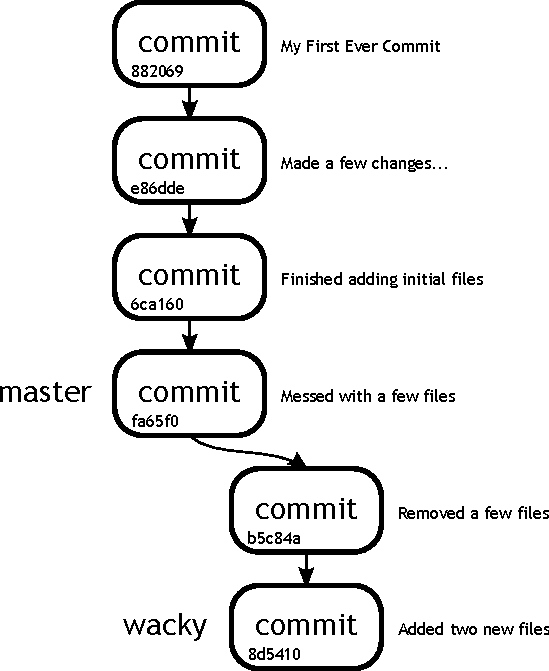
\includegraphics[width=9cm]{images/f-w4-d1.pdf}
\caption{Our first branch}
\end{figure}

So there are really two pointers in our repository at the moment, from a branch point of view.  One of them points to commit \textbf{fa65f0\ldots} and is called \textbf master.  The other is called \textbf{wacky} and points to \textbf{8d5410
\ldots}.  At this point you may be thinking that branches are pretty much the same thing as tags.  Well, they are except for one important fact.  We are going to use our \texttt{git branch} command, with a new parameter, to show us the difference.  Take a look at the output of the following operations.  We have pruned the output of the \texttt{git show} command for brievity.

\begin{Verbatim}[frame=leftline,framerule=1mm,fontsize=\relsize{-3}] 
john@akira:~/coderepo$ git branch -v
  master fa65f06 Messed with a few files
* wacky  8d5140a Added two new files
john@akira:~/coderepo$ git tag v2.0
john@akira:~/coderepo$ git show v2.0
commit 8d5140aa7d2bfc43b225afd2549d180dcb16bef6
...
...
...
\end{Verbatim}

So here we have added a tag in our current branch, \textbf{wacky}, and we can see that the commit id for the tag \textbf{v2.0} points to the commit \textbf{8d5140a}.  We can also see that the branch \textbf{wacky} is currently pointing to the same commit ID, \textbf{8d5140a}.  Now let us add another file in, make a commit and see what happens after this.

\begin{Verbatim}[frame=leftline,framerule=1mm,fontsize=\relsize{-3}] 
john@akira:~/coderepo$ echo "New stuff" > another_file
john@akira:~/coderepo$ git add another_file
john@akira:~/coderepo$ git commit -m 'Added another file'
[wacky f91f31e] Added another file
 1 files changed, 1 insertions(+), 0 deletions(-)
 create mode 100644 another_file
john@akira:~/coderepo$ git show v2.0 
commit 8d5140aa7d2bfc43b225afd2549d180dcb16bef6
...
...
...
john@akira:~/coderepo$ git branch -v
  master fa65f06 Messed with a few files
* wacky  f91f31e Added another file
john@akira:~/coderepo$ 
\end{Verbatim}

How interesting.  The difference between tags and branches now becomes pretty clear.  Whilst a tag always points to the same commit, a branch reference always points to the tip of that branch.  In essence the reference that a branch points to moves as subsequent commits are made.  In doing this, the whole history of the branch can be revealed.  Since we know the latest commit, we also know the parent of that commit and so on and so on.

Since a branch is just a pointer to a commit, adding to it, modifying it and deleting it can be done safely, without destroying any data in another branch.  In short, it will allow us to completely redesign whatever is being stored in the repository without worrying about how it will affect our baseline.

\section{Day 2 - ``Branches galore''}
\subsection{Working with branches}

Now we know about branches in general, we should really learn about how to merge changes from one branch into another.  Branches are fantastic for trying new things out and testing ideas, but if those ideas are successful, we need a way of pulling those changes into our \textbf{master} branch.  Of course we could do it the old fashioned way.  

We could switch into our \textbf{wacky} branch, do a little development, copy the files somewhere else, switch to our \textbf{master} branch, and paste the files over the top.  Now, this is probably the simplest way of merging possible.  In actual fact, this is not really merging at all.  Let us take a litle look at both the command output of a simple merge, explain it a little, and then look at a diagramatic explanation.

\begin{Verbatim}[frame=leftline,framerule=1mm,fontsize=\relsize{-3}] 
john@akira:~/coderepo$ git branch
  master
* wacky
john@akira:~/coderepo$ 
\end{Verbatim}

Firstly we check just to see what branch we are on.  Next we checkout the branch we want our development branch to be merged into.  In this case, we want to merge \textbf{wacky} into \textbf{master} and so we must first checkout the \textbf{master} branch in order to pull in changes from \textbf{wacky}.

\begin{Verbatim}[frame=leftline,framerule=1mm,fontsize=\relsize{-3}] 
john@akira:~/coderepo$ git checkout master
Switched to branch 'master'
john@akira:~/coderepo$ 
\end{Verbatim}

Now we run the actual merge.

\begin{Verbatim}[frame=leftline,framerule=1mm,fontsize=\relsize{-3}] 
john@akira:~/coderepo$ git merge wacky 
Updating fa65f06..f91f31e
Fast-forward
 another_file             |    1 +
 my_first_committed_file  |    1 -
 my_second_committed_file |    1 -
 newfile1                 |    1 +
 newfile2                 |    1 +
 5 files changed, 3 insertions(+), 2 deletions(-)
 create mode 100644 another_file
 delete mode 100644 my_first_committed_file
 delete mode 100644 my_second_committed_file
 create mode 100644 newfile1
 create mode 100644 newfile2
john@akira:~/coderepo$
\end{Verbatim} 

We can see that the first line after our command shows us which commit we are moving from, and then which commit we should end up on.  In this case we are merging from \textbf{fa65f06} to \textbf{f91f31e}.  The line below this is even more important.  This type of merge is called a \emph{fast-forward} merge.  We have not made any changes to our \textbf{master} branch since we began and subsequently finished out development work, and so instead of having to really merge changes, we have literally just fast-forwarded the \textbf{master} branch, to the same point as our \textbf{wacky} one.  Beneath this text, we see more information about just what is included in the merge.  

\begin{Verbatim}[frame=leftline,framerule=1mm,fontsize=\relsize{-3}] 
john@akira:~/coderepo$ git log -n 1
commit f91f31ee594ff9edade7675dd0991b9c0f7c469b
Author: John Haskins <john.haskins@tamagoyakiinc.koala>
Date:   Wed Mar 16 19:21:46 2011 +0000

    Added another file
john@akira:~/coderepo$ git branch
* master
  wacky
john@akira:~/coderepo$ 
\end{Verbatim}

Finally, we just check to see that we are in fact on the master branch and that the latest log message is the one from the point we last left the \textbf{wacky} branch.

Now let us take a quick look at a diagram to see how this change actually affected the commit flow.  We have included tags in this diagram, so that you can see where they point to as well.

\begin{figure}[hbt]
\centering
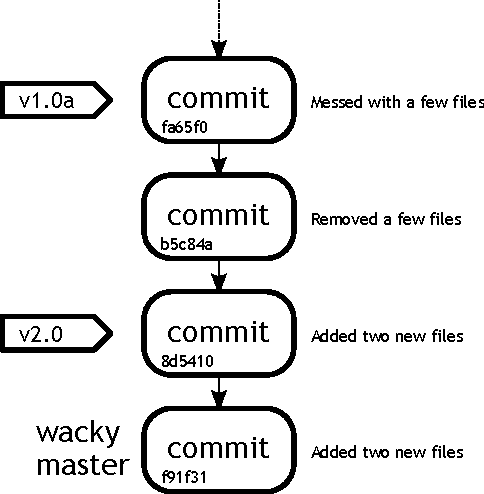
\includegraphics[width=9cm]{images/f-w4-d2.pdf}
\caption{Our first merge}
\end{figure}

\section{Day 3 - ``Tricking the twigs''}
\subsection{Neat ways to work}

There are a number of tricks that we can employ when using branches.  

BRINGING CHANGES TO new BRANCH

DO THE WHOLE AHHH I HAVE STUFF I WANT IN A NEW BRANCH
THEN DO THE SAME WITH A COMMIT
THEN STASH

Before we jump into this, one of the employees at Tamagoyaki has noticed something.

\begin{trenches}
``So John,'' started Rob, ``Just how are we backing up the repository at the moment?''

John thought for a moment before replying.  He knew what Rob was getting at, but he hadn't expected Rob to bring the question up in front of Markus.  In truth he had forgotten all about it.  He turned to Markus.

``I'll be honest Markus.  Currently the repository isn't being backed up, but then we are running in parallel with the old system, so it would be the end of the world if we lost it.''

Markus nodded and smiled.  It seemed that John had gotten away with it for now and with that, Klaus shot Rob a piercing glance.  

``Team,'' began Markus, ``we need a definitive way of backing up the new Git repository, and I'd like it done before the end of the day.''  He pointed at a document on the table.  ``This project document has been approved by Wayne, and in there it states we will have a defined backup strategy.  Please don't let me down.''

\begin{center} * * * \end{center}

``Rob you really got to be careful about things like that,'' Klaus said to one of the younger members of the team.  ``You really showed John up in there.''  

``Yeh,'' said Rob, ``I realise that now.''  He stood with his back against the wall and tapped his fingers against the painted surface.  ``I was wondering, do you think John would let me look at the backup system for him as a way of apologising.''

Klaus smiled, it seemed Rob was finally understanding things, ``Go ask him,'' said Klaus, ``He's so snowed under with the BurnForce release that he'll probably let you implement it too''

``Right'' nodded Rob and off he went.
\end{trenches}

So before we even begin to look at anything like branching, merging or rebasing, we first need to find out how to make a backup of our repository and keep it up to date.  Obviously we could just take the files and copy them, but perhaps a better way of doing this is to clone our repository using the \texttt{git clone} command.  Cloning a repository basically means creating an exact copy of the data in an alternative location.  Well, that's what cloning means isn't it?

The git clone tool doesn't just copy the data though, it does several other things.  Let us create a clone of our test repository 

%branches
%merge
%remote tracking
%Itt section about not having anything backed up

%Parallel devving - ie...use both git and old for a while

% git show v1.0.0^{tree}
